\section{Signal Selection}
\label{sec:stop_strategy}

%%%%%%%%%%%%%%%%%%%%%%%%%%%%%%%%%%%%%%%%%%%%%%%%%%%%%%%%%%%%%%%%%%%%%%%%%%%
%%%%%%%%%%%%%%%%%%%%%%%%%%%%%%%%%%%%%%%%%%%%%%%%%%%%%%%%%%%%%%%%%%%%%%%%%%%
%%%%%%%%%%%%%%%%%%%%%%%%%%%%%%%%%%%%%%%%%%%%%%%%%%%%%%%%%%%%%%%%%%%%%%%%%%%
%
% RJR
%
%%%%%%%%%%%%%%%%%%%%%%%%%%%%%%%%%%%%%%%%%%%%%%%%%%%%%%%%%%%%%%%%%%%%%%%%%%%
%%%%%%%%%%%%%%%%%%%%%%%%%%%%%%%%%%%%%%%%%%%%%%%%%%%%%%%%%%%%%%%%%%%%%%%%%%%
%%%%%%%%%%%%%%%%%%%%%%%%%%%%%%%%%%%%%%%%%%%%%%%%%%%%%%%%%%%%%%%%%%%%%%%%%%%
\subsection{The Recursive Jigsaw Reconstruction}
\label{sec:stop_rjr}

The \stopone search presented here makes use of of a high-level event reconstruction
technique referred to as the `Recursive Jigsaw Reconstruction' (RJR) technique~\cite{RecursiveJigsaw}.
This technique is a generalisation of the methods introduced in Ref.~\cite{SuperRazor}, referred
to as the `Super Razor'.

The RJR technique takes the measured information in an event --- the observable objects and their
four momenta, as well as the missing transverse momentum --- and, through a series of assumptions
and algorithms is able to reorganize those objects in such a way as to be interpreted as `fitting' into
a user-specified, or rather user-\textit{imposed}, decay tree.
Indeed, the technique's name derives from the mehods it employs to perform this reorganization.
The `recursion' implied in the technique's name refers to the way in which its rules and algorithms
are implemented in order to \textit{navigate} through the decay tree: stepping through the decay
tree one level at at time, using information only from the current reference frame associated with
the object in the decay tree in that level, to determine the properties of the subsequent ones.
This effectively means that conclusions drawn at the `upper levels' of the decay about the kinematic
properties of the particles present are not lost or altered as one traverses further down the decay chain.
The `jigsaw' in the technique's name refers to the sets of rules and/or algorithms that are applied ---
so-called `Jigsaw rules' --- in order to either piece together or break apart the reconstructed
event provided the kinematic information (lab-frame four-vectors) that the user has provided as input
to the decay tree assumption.

As an illustrative example of this decay tree `fitting', consider the \ttbar~and $\stopone \rightarrow b \chinoonepm$
decays illustrated in Figure~\ref{fig:rjr_ttbar_bcn}, which provides an example of an RJR decay tree imposition.
As will be outlined later, the RJR technique determines the relative velocities (boosts) between
the different states or rest-frames present in a given RJR decay tree.
These boosts between frames are illustrated diagrammatically as the black lines in the lower portion of
Figure~\ref{fig:rjr_ttbar_bcn} connecting the various states, both intermediate (`Decay States')
and final (`Visible States' or `Invisible States'), which are represented as the circles.
Although the two processes differ, they both fit topologically the RJR decay tree in Figure~\ref{fig:rjr_ttbar_bcn}.
In both cases, the final state is composed of two $b$-tagged jets, two leptons, and missing transverse
momentum and one can intuitively see how to allocate these objects' four-momenta to the states in the
RJR decay tree: the $V_{1\,(a,b)}$ states
are the $b$-tagged jets, the $V_{2\,(a,b)}$ states are the leptons, and the $I_{a,b}$ represent
the neutrinos (plus the LSPs in the case of the $\stopone \rightarrow b \chinoonepm$ signal).
Although the two processes may fit the same RJR tree, they are of course quite different kinematically
(e.g. the $I_{a,b}$ states for $\stopone \rightarrow b \chinoonepm$ are composed of additional
\textit{massive} particles in addition to the neutrinos) and any variable derived using the four-vectors
derived from this decay tree imposition has the potential to tease out these differences
between the signal and background processes.

\begin{figure}[!htb]
    \begin{center}
        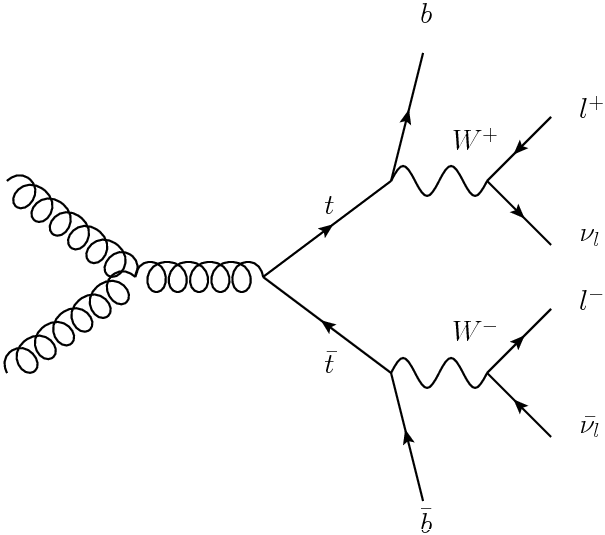
\includegraphics[width=0.4\textwidth]{figures/search_stop2l/strategy/fgraph_ttbar}
        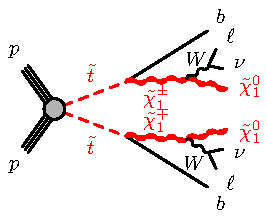
\includegraphics[width=0.4\textwidth]{figures/search_stop2l/strategy/fgraph_stop_bCN}
        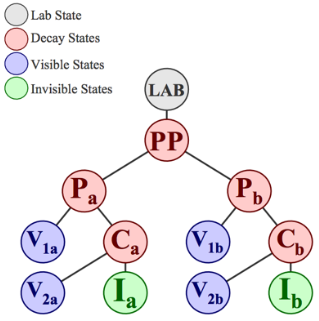
\includegraphics[width=0.5\textwidth]{figures/search_stop2l/strategy/RJRtree_generic_PPviaC}
        \caption{
            An example of an RJR decay tree interpretation of physics processes.
            The RJR decay tree (\textit{\textbf{bottom}}) can be fit to both the \ttbar~decay
            (\textit{\textbf{upper left}}) or the $\stopone \rightarrow b \chinoonepm$ process (\textit{\textbf{upper right}}).
            Each of the upper processes \textit{topologically} matches that of the RJR decay tree, but
            the underlying differences in their kinematics means that kinematic observables derived
            from this RJR decay tree may provide means of discrimination between the two.
            Each circle in the RJR decay tree represents a reconstructed reference frame,
            characterised by its own four-vector information.
        }
        \label{fig:rjr_ttbar_bcn}
    \end{center}
\end{figure}

\FloatBarrier
%%%%%%%%%%%%%%%%%%%%%%%%%%%%%%%%%%%%%%%%%%%%%%%%%%%%%%%%%%%%%%%%%%%%%%%%%%%
%%%%%%%%%%%%%%%%%%%%%%%%%%%%%%%%%%%%%%%%%%%%%%%%%%%%%%%%%%%%%%%%%%%%%%%%%%%
%%%%%%%%%%%%%%%%%%%%%%%%%%%%%%%%%%%%%%%%%%%%%%%%%%%%%%%%%%%%%%%%%%%%%%%%%%%
%
% RJR FOR THREE BODY
%
%%%%%%%%%%%%%%%%%%%%%%%%%%%%%%%%%%%%%%%%%%%%%%%%%%%%%%%%%%%%%%%%%%%%%%%%%%%
%%%%%%%%%%%%%%%%%%%%%%%%%%%%%%%%%%%%%%%%%%%%%%%%%%%%%%%%%%%%%%%%%%%%%%%%%%%
%%%%%%%%%%%%%%%%%%%%%%%%%%%%%%%%%%%%%%%%%%%%%%%%%%%%%%%%%%%%%%%%%%%%%%%%%%%

The RJR decay tree imposed in the present analysis searching for the three-body decay
of the \stopone quark is presented in Figure~\ref{fig:rjr_stop}.
The visible system ($V_a + V_b$) is provided only the two leptons in the event.
The invisible system ($I_a + I_b$) is provided the missing transverse momentum.

\begin{figure}[!htb]
    \begin{center}
        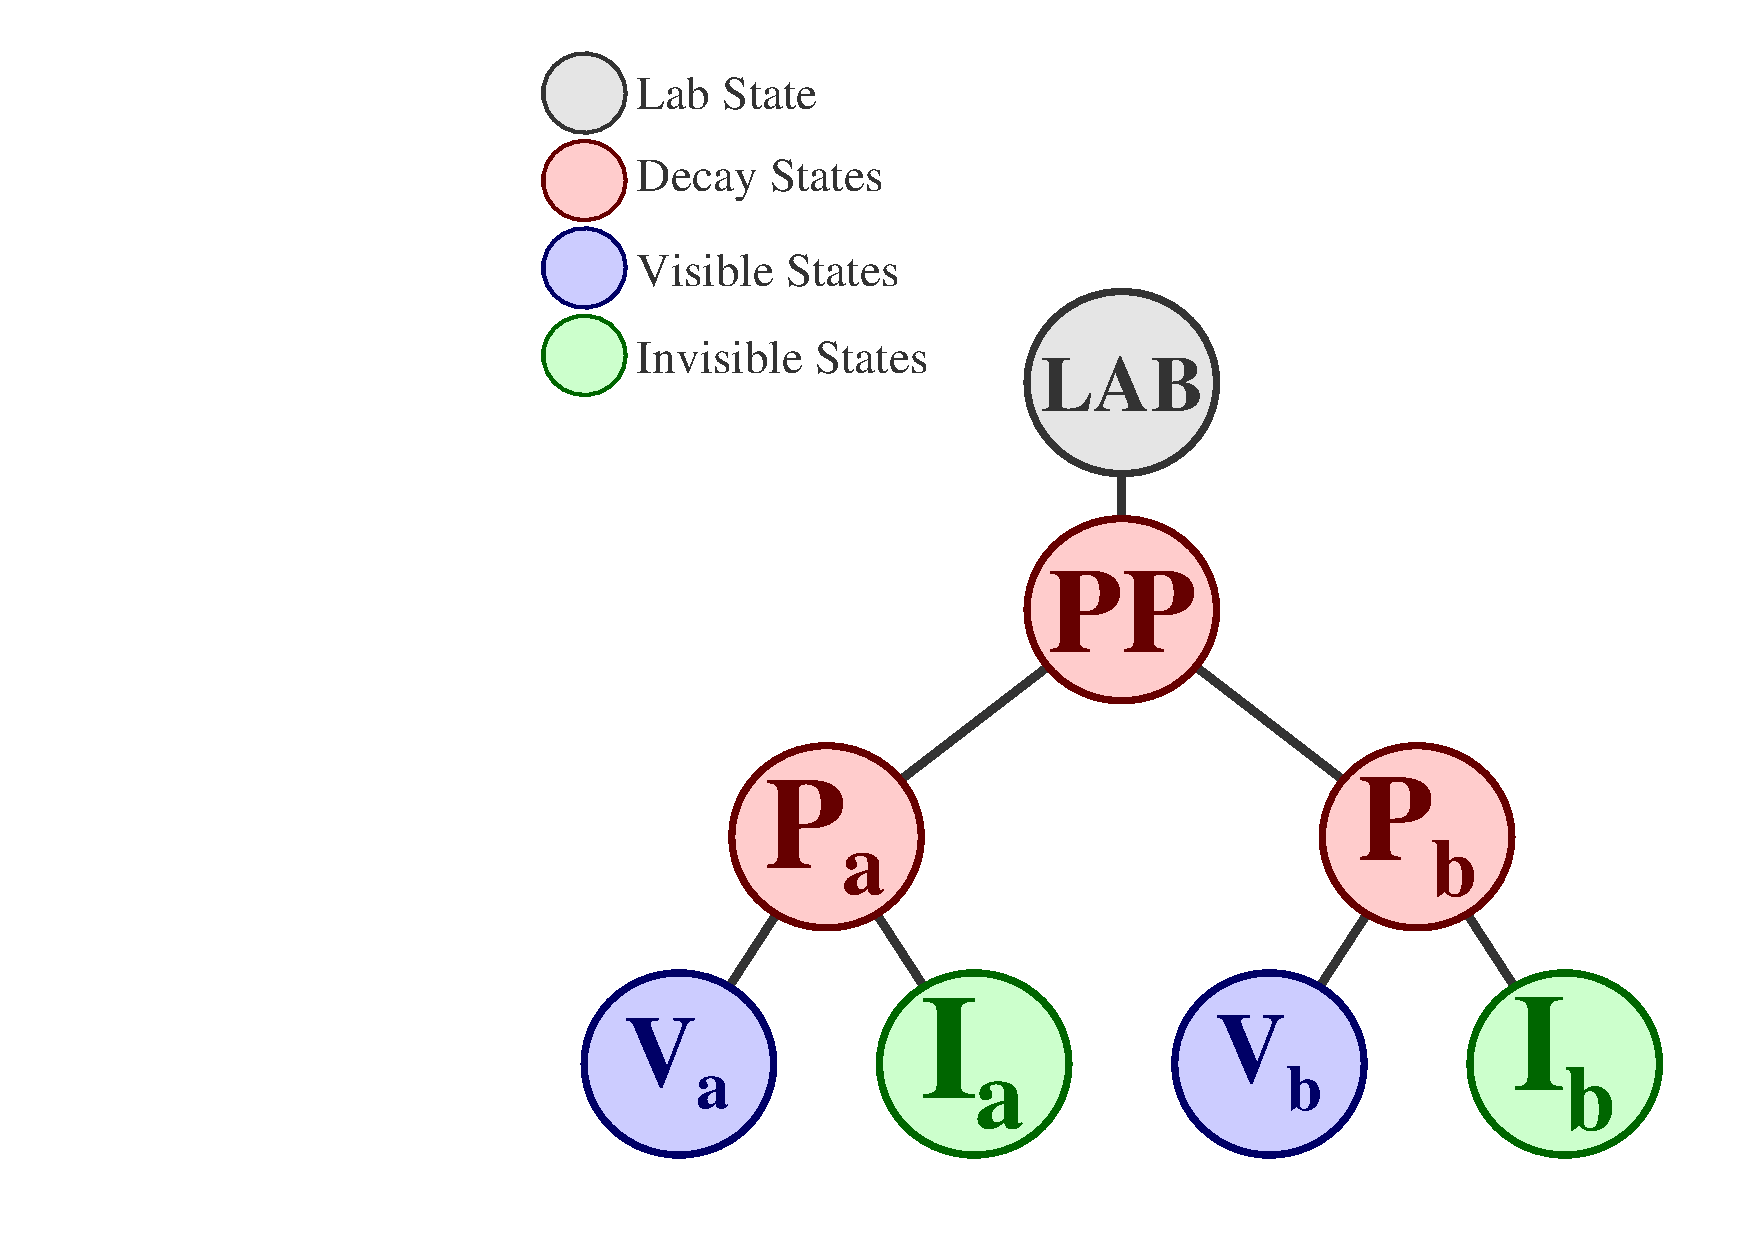
\includegraphics[width=0.6\textwidth]{figures/search_stop2l/strategy/RJRtree_DiSparticle}
        \caption{
            RJR decay tree assumption used in the 2015+2016 analysis searching for the
            three-body decay of the \stopone quark, $\stopone \rightarrow b W \ninoone$.
            It is the most general decay tree for $R$-parity conserving SUSY scenarios in
            which pair-produced sparticles ($P_a$ and $P_b$) each decay to visible states ($V_a$ and $V_b$)
            and invisible states ($I_a$ and $I_b$).
            Each of the final states ($V_i$ and/or $I_i$) may, in principle, be composed of multiple particles.
            In the present analysis, only the two leptons in the event are provided as inputs to the $V_i$ and both
            are required to be non-empty (i.e. $V_a$ is one of the leptons, $V_b$ the other).
            The missing transverse momentum in the event is decomposed via a set of Jigsaw Rules into the
            states $I_a$ and $I_b$.
        }
        \label{fig:rjr_stop}
    \end{center}
\end{figure}

The RJR decay tree in Figure~\ref{fig:rjr_stop} is the most general RJR decay tree one can make for
targetting $R$-parity conserving SUSY models.
This decay tree makes the least number of assumptions on the decay of the pair-produced sparticles and
their children (if any).
This is beneficial, as developing a search (whose a-priori intent is for discovery of new physics)
that is largely dependent on the model assumed for designing the analysis' selection criteria
greatly limits the applicability and scope of that search.
For example, one can imagine using the decay tree of Figure~\ref{fig:rjr_ttbar_bcn} also for the three-body
decays considered in the present search, $\stopone \rightarrow b W \ninoone$.
However, the decay tree in Figure~\ref{fig:rjr_ttbar_bcn} assumpes that there is enough information to
kinematically separate the $b$-tagged jets and leptons into the $V_{1(a,b)}$ and $V_{2(a,b)}$ states,
respectively, therefore requiring at least four visible objects to be reconstructed.
As discussed in Section~\ref{sec:stop_final_state}, this is not the case for the three-body decays
of the \stopone relevant for the present analysis and so Figure~\ref{fig:rjr_ttbar_bcn} is not well-suited
for this search.
What we want, in the end, is a means to separate from the background the presence of an $R$-parity conserving
SUSY signal while making as few assumptions as possible.

As mentioned, the goal of the RJR technique is to provide a full accounting of all of the states specified by the
user in the imposed RJR decay tree; or, at least a close and/or optimal approximation of them.
Unfortunately, it is in generall impossible to do this as a result of the presence of multiple weakly interacting
particles in the final state and, less generally, because of combinatoric ambiguities
that make it difficult to assign objects to specific locations in the decay (e.g. associating $b$-jets to
the correct side of the decay).
The RJR technique and its so-called Jigsaw Rules provide a means to systematically resolve these unknowns
on an event-by-event basis.

In order to resolve combinatoric ambiguities amongst the reconstructed visible objects so that they may
be grouped `correctly', one can employ a Jigsaw Rule for performing a recursive partitioning
of the visible objects until that grouping which minimizes the visible mass of each side of a decay vertex is found.
This is not necessarily the true grouping, but it is a method that is found to reproduce well, on average,
the correct grouping of objects.

In the RJR decay tree used in the search for $\stopone \rightarrow b W \ninoone$, illustrated
in Figure~\ref{fig:rjr_stop}, there are 6 under-constrained degrees-of-freedom (DOF) due to the
weakly interacting particles/missing transverse momentum.
These are (2 DOF for each) as follows:
\begin{itemize}
    \item The longitudinal momenta of the $I_i$ states: $p_{I_i,z}$
    \item The splitting of the missing transverse momentum between the $I_i$ states: $\bm{p}_{I_a,T} + \bm{p}_{I_b,T} = \bm{E}_T^{\text{miss}}$
    \item The mass of the di-invisible system composed of $I_a$ and $I_b$: $m_I$ ($m_{I_a}$ and $m_{I_b}$)
\end{itemize}
The RJR technique sets out to provide values for these unknowns through assumptions (constraints) that it makes
for determining the relative velocities (boosts) between rest-frames indicated by the circles in Figure~\ref{fig:rjr_stop}.
The recursive element of the technique is most obvious in this respect: the algorithm moves from
the first known reference frame (the lab frame) and traverses down the decay tree using information
only from the current frame to determine the boosts for moving into the next reference frame.
That is, with respect to Figure~\ref{fig:rjr_stop}, information only from the lab frame
is used to move to the $PP$ (center-of-mass, COM) frame and information from this COM frame
is used to move to either of the respective $P_i$ frames.
There are specific Jigsaw Rules at each step of this navigating of the RJR decay tree that determine
\textit{how} the information in each of these frames is used simultaneously to move to the next
and to provide estimates of the under-constrained DOF mentioned above.

The first step that the RJR technique takes in constructing the boosts relating the reference frames is to
determine the mass of the invisible system, $m_I$, composed of the states $I_a$ and $I_b$.
This information is required to be able to consistently perform boosts between the reference frames while
keeping each side, or \textit{hemisphere}, of the decay balanced against the other.
This means that, generally, the di-invisible system will have non-trivial opening angles between the $I_i$
states in order to balance the visible system frame-by-frame.
This means that it will attain a mass\footnote{From special relativistic mechanics, the mass of a system comprised
of two subsystems, 1 and 2, is generally given by $m_{12}^2 = m_1^2 + m_2^2 + 2(E_1E_2 - |\vec{p}_1| |\vec{p}_2| \cos \theta_{12})$,
where $\theta_{12}$ is the opening angle between $\vec{p}_1$ and $\vec{p}_2$.}
To satisfy this balancing requirement, the RJR technique takes for $m_I$ the smallest Lorentz-invariant
mass consistent with the input lab-frame observables that will accomodate the subsequent boosts and also prevent
the states $I_i$ from becoming tachyonic.
For the decay tree in Figure~\ref{fig:rjr_stop} this turns out to be,
\begin{align}
    m_I^2 = m_V^2 - 4m_{V_a} m_{V_b},
    \label{eq:rjr_invisible_mass}
\end{align}
where $V$ refers to the total visible system comprised of $V_a$ and $V_b$.

Next, the RJR technique determines the boost from the lab to the $PP$ (COM) frame.
To determine this boost, we must determine the longitudinal momentum of the invisible system, $p_{I,z}^{\text{Lab}}$,
which is one of the under-constrained DOF.
The RJR technique chooses this value such that the rapidity of the visible and invisible systems are equal.
This choice results in our choice of the $PP$ (COM) reference frame being a longitudinally boost-invariant
choice, meaning that all subsequent observables derived in the RJR decay tree will also be
longitudinally boost-invariant.
Additionally, one can see that this also forces the mass of the $PP$ system, $m_{V+I}$, to
take its minimum value.\footnote{This is een using the previous footnote and knowledge that $\vec{E}_T^{\text{miss}}$
must balance the visible system's transverse momentum.}

With the longitudinal momentum of the invisible system determined, along with its mass, we have
the expression for the boost relating the lab frame to the $PP$ (COM) frame:
\begin{align}
    \vec{\beta}_{PP}^{\,\text{LAB}} = \frac{
        \vec{p}_{PP}^{\text{LAB}}
    }
    {
        E_{PP}^{\text{LAB}}
    }
    = \frac{
        \vec{p}_V^{\,\text{LAB}} + \vec{p}_I^{\,\text{LAB}}
    }
    {
        E_V^{\text{LAB}} + \sqrt{ |\vec{p}_I^{\,\text{LAB}} |^2 + m_I^2 }.
    }
    \label{eq:rjr_lab_boost}
\end{align}
The boost in Equation~\ref{eq:rjr_lab_boost} affords provides us the observables in the $PP$ (COM)
reference frame.
We must use information in this frame to determine how to move to the individual sparticle frames, $P_i$.
This will provide us with the last set of information regarding how the missing transverse momentum
is to be shared between the states $I_i$.
Here, the RJR technique makes the assumption that $m_{V_a} = m_{V_b}$, which, in the context of the processes
considered, is reasonable.
As we are in the COM frame, this choice for the masses of the $V_i$ states dicates that the boosts of each of their
individual reference frames be equal in magnitude and anti-parallel.
For our decay tree, a possible solution for this is chosen to be:
\begin{align}
    \vec{\beta}_{P_i}^{\,PP} = \frac{
        \vec{p}_{V_a}^{\,PP} - \vec{p}_{V_b}^{\,PP}
    }
    {
        E_{V_a}^{PP} + E_{V_b}^{PP}.
    }
    \label{eq:rjr_pi_boost}
\end{align}
Under this boost, all observables subsequently defined are \textit{contra-boost invariant}, meaning that,
as in the case for the longitudinal boost invariance described previously, all observables
are therefore insensitive (on average) to the fact that this boost from the $PP$ (COM) frame to the $P_i$
frames is not necessarily the true boost.
Indeed, this final contra-boost invariance is the main motivation behind the structure of Equation~\ref{eq:rjr_pi_boost}.

Now that we have the boost $\vec{\beta}_{P_i}^{\,PP}$ to the $P_i$ frames, one can determine the splitting of invisible
momentum by requiring $\vec{p}_{V_i}^{\,P_i} + \vec{p}_{I_i}^{\,P_i} = 0$, which
is the final under-constrained DOF of the RJR decay tree relevant to the analysis being presented.

With the application of the RJR technique, then, all of the unknowns in the event are thus determined
(approximately), and one has access to kinematic information (four vectors) for every level of the RJR decay tree
that has been imposed (Figure~\ref{fig:rjr_stop}).


\subsection{Discriminating Observables}
\label{sec:stop_variables}

\subsection{Signal Region Definitions}
\label{sec:stop_signal_region}
